% !TEX root = ../thesis-example.tex
%
\chapter{Interface sensible / hardware}
\label{ch:interfaces}

\cleanchapterquote{Komponieren heißt: über die Mittel nachdenken.\\
Komponieren heißt: ein Instrument bauen.\\
Komponieren heißt: nicht sich gehen, sondern sich kommen lassen.\\
.}{Helmut Lachenmann}{1986}

\cleanchapterquote{Fingers are not to be despised: they are great inspirers, and, in contact with a musical instrument, often give birth to subconscious ideas which might otherwise never come to life.}{Igor Stravinsky}{1936}


\vspace{-1em}
\begin{itemize}[noitemsep]
\item Faire évoluer une interface en la raffinant (De Laubier, VG).
\item Faire évoluer une interface en rajoutant des choses (Patricia Dallio)
\item Faire évoluer en supprimant des choses (Dumaux)
\item Partir de l'objet (Patrick Saint Denis)
\end{itemize}

%----------------------------------------------------------------------------------------------------------
\section{Interface gestuelle ou interface sensible?}
Il est souvent question d'\textit{interface gestuelle} lorsqu'on pense aux IHM utilisées pour l'interaction musicale. Pourtant, si le geste occupe une part importante de l'interaction musicale, les interfaces de jeu ne se restreignent pas nécessairement à la captation du geste : elle peuvent être sensible à la température, la lumière \footnote{Voir par exemple les œuvres \textit{Light Thing} de Leaf Cutter John (\url{https://youtu.be/2jIlLHfSEfs}), ou encore \textit{Light Music} de Thierry de Mey}, à la couleur, et réagir de manière générale à différentes conditions environnementales 

Par ailleurs, le geste possède un certain nombre de qualités qui ne sont pas captées par l'interface, alors qu'elle sont effectivement vues et ressenties par le musicien et par le public, et contribuent ainsi à la performance.

Enfin, le "geste" qui vient contrôler les processus sonores dans les DMIs peut être de nature virtuelle, prendre la forme de motifs pré-enregistrés qui peuvent être issus de toute sorte de source de données interprétées en tant que flux temporels, tels que peut -être le cas dans la sonification de données ou l'utilisation de modèles intermédiaire. Cet aspect là se décrit plus en détail dans le chapitre \ref{ch:algorithms}.

Il semble ainsi préférable d'interface sensible, en tant que leur caractéristique commune est l'usage de capteurs (\textit{sensors}).

%%%%%%%%%%%%%%%%%%%%%%%%%%%%%%%%%%%%%%%%%
\section{Interface pour composer/interpréter/improviser en live}
Articulation entre grandes formes et immédiateté : la gestion du temps de l’interaction à différentes échelles.
La performance musicale avec un DMI permet d’articuler une partie compositionnelle (échelle de temps longue) et une partie interprétation/improvisation (immédiateté de l’instant). 
Quelle design d’interface permet de répondre à l’articulation de ces 2 pôles ? 

%%%%%%%%%%%%%%%%%%%%%%%%%%%%%%%%%%%%%%%%%
\section{Qualité ergodynamiques}
%----------------------------------------------------------------------------------------------------------
\subsection{Ergodynamisme}
cf. définition de Thor Magnusson
choix des capteurs, latence
agencement de l’interface, représentation visuelle, repères tactile, frettage

%----------------------------------------------------------------------------------------------------------

\subsection{facteur de forme et topologie: héritage et transpositions}

%----------------------------------------------------------------------------------------------------------
\subsection{retour audio-tactile}
Intégration de HP tactile
Spatialisation ou diffusion ad-hoc
Travail avec Pascale Criton à la maison des aveugles


%%%%%%%%%%%%%%%%%%%%%%%%%%%%%%%%%%%%%%%%%
\section{Généalogie d’une interface de DMI}
\label{sec:interfaces:sec1}

Filigramophone : évolution depuis la tablette graphique simple, tablette augmentée, écran multitouch augmenté, intégration de Bela…

De la simple tablette graphique à l’écran multitouch augmenté de capteurs, histoire de l’évolution d’une interface pour la performance électroacoustique.
La conception d’une nouvelle interface pour la performance musicale est une tâche complexe, nécessitant de nombreux aller-retours entre conception, fabrication et pratique musicale. Le filigramophone est une interface qui a connu plusieurs versions, suffisamment différentes pour avoir envie de leur donner un nouveau nom à chaque fois et suffisamment similaire pour y voir la continuité d’un seul et même instrument.

%----------------------------------------------------------------------------------------------------------
\subsection{origine : la tablette graphique}
La tablette graphique (nommément un modèle Sapphire de Wacom) a été l’interface originelle qui a servi de base au filigramophone. J’ai commencé à l’utiliser suite à son utilisation dans le cadre de la Méta-Mallette\footnote{Logiciel pour la pratique collective de musique par ordinateur développé par l’association Puce Muse.}. La raison de ce choix est que la tablette graphique offre une interface relativement bon marché (donc déployable en nombre) qui permet un contrôle assez fin de la synthèse sonore.
Un certain nombre de musiciens, compositeurs et concepteurs de NIME l’ont adopté pour leurs projets \cite{zbyszynski_ten_2007}, et Nicolas d’Alessandro a consacré une partie de son travail de thèse \cite{dalessandro_realtime_2009} à ce sujet.

La tablette graphique permet de bénéficier de l’expertise du geste d’écriture et de dessin.


%----------------------------------------------------------------------------------------------------------
\subsection{augmentation de la tablette graphique}
ajout de piezo et HP tactile pour une réponse immédiate
ajout de MPD pour le changement de comportement
ajout de carte/frettage de la tablette (aux crayon et feutres)

Problème de devoir tout démonter l'instrument pour changer la feuille de frettage. => solution graphique ?

%-------------------------- Figure : filigramophone ----------------------------------
\begin{figure}[!htbp]
	\includegraphics[width=\textwidth]{gfx/filigramophone/filigramophone_overview.jpg}
	\caption{filigramophone - vue d'ensemble, débranchée}
	\label{fig:interface:filigramophone}
\end{figure}

%----------------------------------------------------------------------------------------------------------
\subsection{de la tablette à l'écran graphique multitouch}
%-------------------------- Figure : xypre ----------------------------------
\begin{figure}[!htbp]
	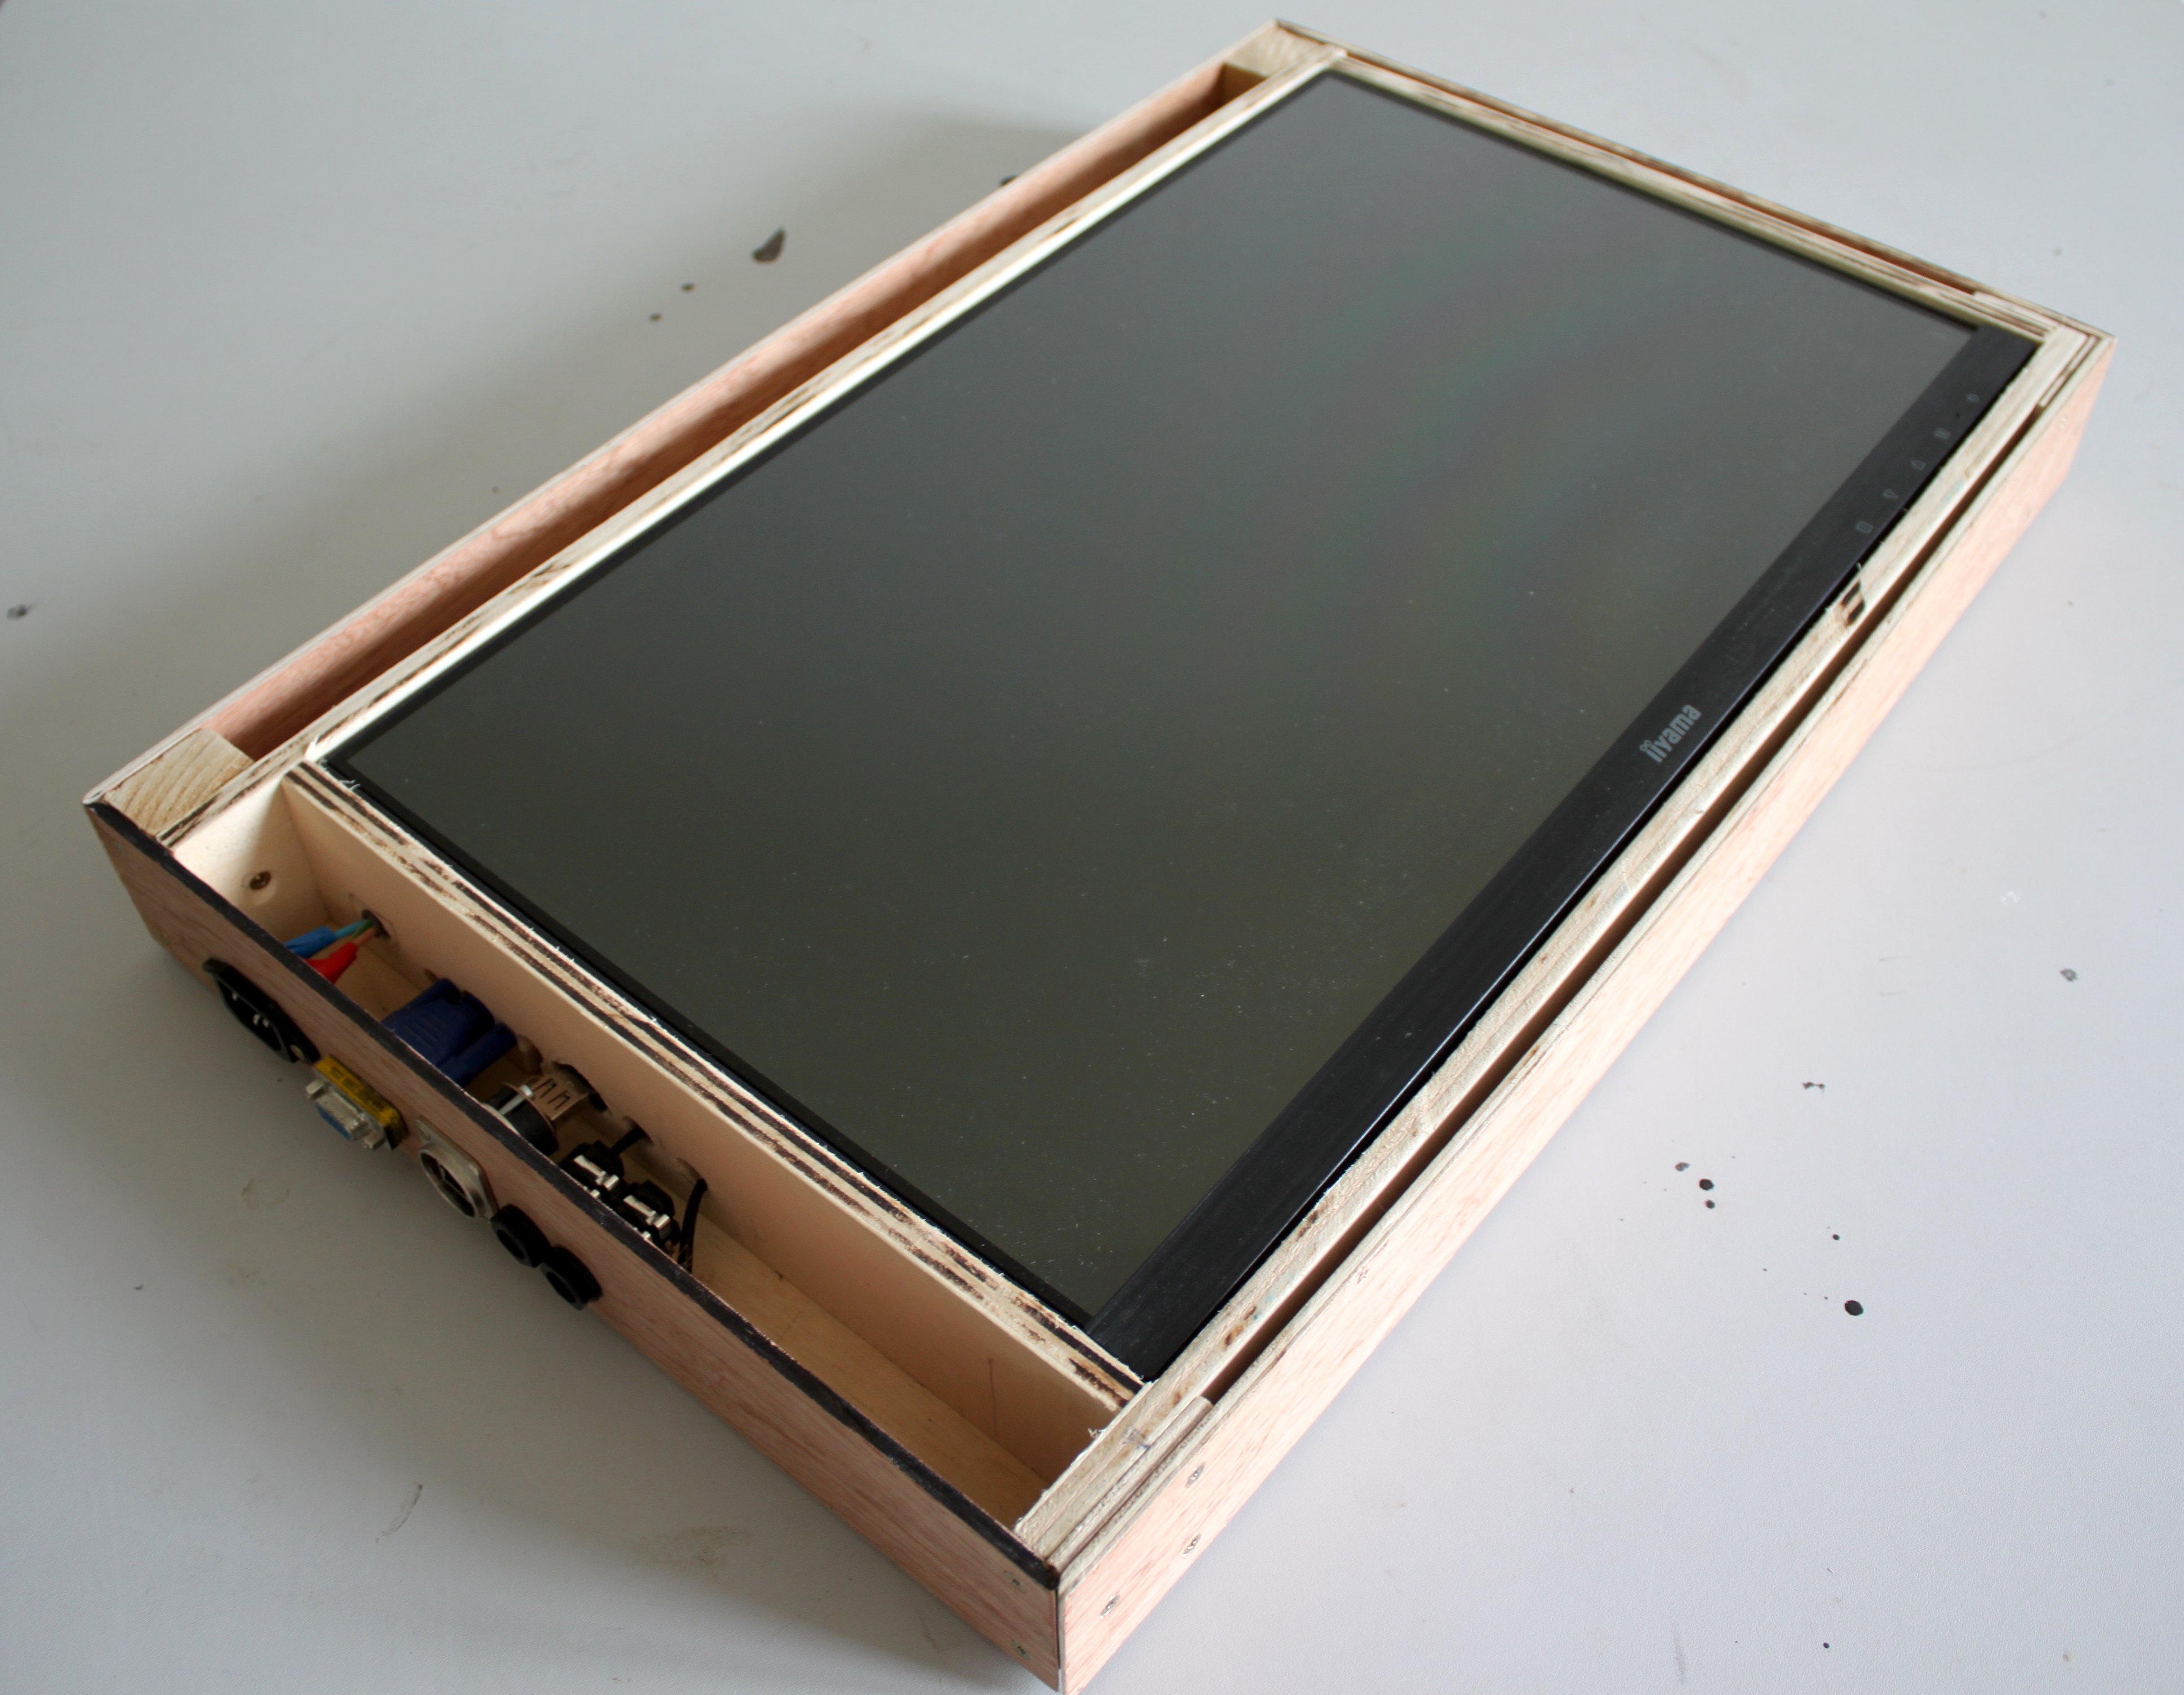
\includegraphics[width=\textwidth]{gfx/xypre/xypre_overview_unplugged.jpg}
	\caption{xypre - vue d'ensemble, débranchée}
	\label{fig:interface:xypre}
\end{figure}

%%%%%%%%%%%%%%%%%%%%%%%%%%%%%%%%%%%%%%%%%
\section{Conclusion}
\label{sec:interfaces:conclusion}


\section*{extra material}

Classification des controleurs gestuels dans \cite{wanderley_controle_1999}:
\vspace{-1em}
\begin{itemize}[noitemsep]
\item \textbf{Instrument-like controllers},where the input device design tends to reproduce each feature of an existing (acoustic) instrument in detail. Many examples can be cited, such as electronic keyboards, guitars, sax- ophones, marimbas, and so on.
\item \textbf{Instrument-inspired controllers} that although largely inspired by the existing instrument’s design, are conceived for another use [62]. Fig. 3 presents one example of such controller, the SuperPolm violin developed by S. Goto, A. Terrier, and P. Pierrot [63], [64], where the input device is loosely based on a violin shape, but is used as a general device to control granular synthesis. => emprunts variés de formes et de fonctions.
\item \textbf{Extended instruments} are instruments augmented by the addition of extra sensors [58], [65]. Commercial augmented instruments included the Yamaha Disklavier, used, for instance, in pieces by J.-C. Risset[66], [67]. Other examples include the flute [68]–[70] and the trumpet [71]–[73], but any existing acoustic instrument may be extended to different degrees by the addition of sensors.
\item \textbf{Alternate controllers} (see, e.g., Fig. 4), whose design does not follow that of an established instrument. Some examples include the Hands [52], graphic drawing tablets [74] (cf. Fig. 5), etc. For instance, an unorthodox gestural controller using the shape of the oral cavity has been proposed in [75].
\end{itemize}

These controllers can furthermore be classified into dif- ferent categories.
\begin{itemize}[noitemsep]
\item \textbf{Touch, expanded range, or immersive} controllers [76], depending on the amount of physical contact required from the performer. Mulder also [76] separates immersive controllers into internal, external, and symbolic controllers according to the possibilities of visualization of the control surface. In a different approach, Piringer [77] classifies immmersive controllers into partial or completely immersive controllers.
\item \textbf{Individual or collaborativecontrollers}[78],depending on whether the instrument is performed by one or mul- tiple performers at one time.
\item \textbf{Metaphorical} or \item{ad hoc} controllers, and so on.
\end{itemize}